
\section{Experiments}


\subsection{Benchmarking}

\begin{figure}[htbp]
    \centering
    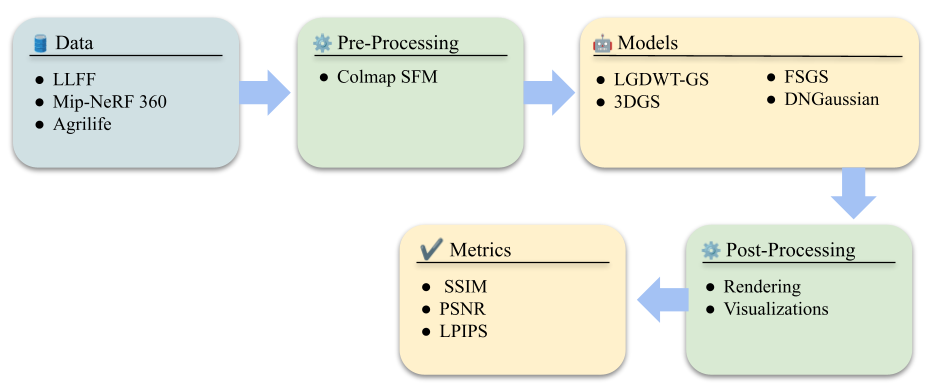
\includegraphics[width=\linewidth]{sections/image/fsgs_benchmarking.png}
    \caption{Few-shot 3DGS benchmarking tool overview. The overall framework and figure is adapted from Anomalib~\cite{akcay2022anomalib}.}
    \label{fig:benchmark}
\end{figure}


We introduce an end-to-end benchmarking pipeline for few-shot 3D reconstruction that unifies data processing, training, and evaluation across multiple Gaussian Splatting baselines. While existing frameworks such as Nerfstudio~\cite{tancik2023nerfstudio} simplify NeRF-style experimentation, they do not yet provide native support for few-shot Gaussian Splatting workflows or standardized evaluation under sparse-view conditions. Our system uses common multi-view datasets and executes a unified SfM stage using COLMAP to ensure consistent camera poses and sparse geometry across all experiments. On top of this shared foundation, the pipeline supports the training of multiple few-shot Gaussian Splatting variants, including 3DGS~\cite{kerbl20233d}, FSGS~\cite{zhu2024fsgs}, and DNGaussian~\cite{li2024dngaussian}, using a common configuration and logging interface.

The benchmarking package is fully modular, allowing new datasets and new Gaussian Splatting methods to be registered through a unified API without re-engineering the environment or modifying existing pipelines. This design enables a one-install, many-model workflow with a fixed data layout, standardized metrics, and consistent evaluation protocols. As a result, comparisons across models, scenes, and random seeds become fair, repeatable, and reproducible, minimizing environment-dependent variability and facilitating reliable analysis of few-shot 3D reconstruction performance.

\subsection{Quantitative Results}

We evaluate the proposed framework on standard benchmarks including LLFF~\cite{mildenhall2019llff}, MipNeRF360~\cite{barron2022mipnerf360}, and our controlled greenhouse multispectral dataset. The evaluation is designed to assess reconstruction quality under varying levels of view sparsity and spectral diversity. All models are trained on a single NVIDIA A100 GPU. Despite its efficiency, the proposed LGDWT-GS pipeline converges in under three minutes per scene while achieving state-of-the-art performance across sparse-view, dense-view, and multispectral settings.

Although the proposed framework supports arbitrary numbers of input views, we report results under representative configurations that are commonly adopted in prior work. Specifically, we evaluate on LLFF using three input views, which is a standard few-shot setting. For MipNeRF360, we report results using 24 input views, which is widely treated as a few-shot configuration due to the dataset’s complex geometry and wide viewpoint variation. For the greenhouse dataset, we adopt a fixed few-shot setting with ten views per plant, reflecting realistic agricultural capture conditions.

Table~\ref{tab:llff_comparison} shows that LGDWT-GS improves performance significantly on the three-view LLFF dataset. These results confirm that frequency supervision prevents the overfitting and structural errors often seen in sparse-view training. LGDWT-GS also consistently outperforms DNGaussian, suggesting that frequency control offers benefits that geometry modeling alone cannot provide. Additionally, our method achieves higher scores than NeRF-based methods like RegNeRF and FreeNeRF. This proves that enforcing consistency in the frequency domain preserves both global structure and fine details, even with very few views.

Table~\ref{tab:mipnerf_comparison} presents results on MipNeRF360 using 24 input views. Even with more images, this dataset remains difficult due to complex scenes and wide angles. Under these conditions, LGDWT-GS achieves the highest overall scores. The strong performance against DNGaussian shows that frequency supervision is effective beyond just sparse data. It ensures stable reconstruction across both limited-view and complex multi-view scenarios.


\begin{table}[h!]
\centering
\caption{Comparison on LLFF (3-View). Metrics include PSNR (dB) $\uparrow$, SSIM $\uparrow$, and LPIPS $\downarrow$.}
\resizebox{0.7\linewidth}{!}{
\begin{tabular}{lccc}
\hline
Method & PSNR $\uparrow$ & SSIM $\uparrow$ & LPIPS $\downarrow$ \\
\hline
Mip-NeRF360 & 15.22 & 0.351 & 0.540 \\
DietNeRF    & 13.86 & 0.305 & 0.578 \\
RegNeRF     & 18.66 & 0.535 & 0.411 \\
FreeNeRF    & 19.13 & 0.562 & 0.384 \\
SparseNeRF  & 19.07 & 0.564 & 0.392 \\
3DGS        & 16.94 & 0.488 & 0.402 \\
DNGaussian  & 19.73 & 0.669 & 0.301 \\
LGDWT-GS (ours) & \textbf{20.46} & \textbf{0.726} & \textbf{0.279} \\
\hline
\end{tabular}}
\label{tab:llff_comparison}
\end{table}


\begin{table}[h!]
\centering
\caption{Comparison on MipNeRF-360 (24-View). Metrics include PSNR (dB) $\uparrow$, SSIM $\uparrow$, and LPIPS $\downarrow$.}
\resizebox{0.7\linewidth}{!}{
\begin{tabular}{lccc}
\hline
Method & PSNR $\uparrow$ & SSIM $\uparrow$ & LPIPS $\downarrow$ \\
\hline
Mip-NeRF360 & 19.78 & 0.530 & 0.431 \\
DietNeRF    & 19.11 & 0.482 & 0.452 \\
RegNeRF     & 20.55 & 0.546 & 0.398 \\
FreeNeRF    & 21.04 & 0.587 & 0.377 \\
SparseNeRF  & 21.13 & 0.600 & 0.389 \\
3DGS        & 19.93 & 0.588 & 0.401 \\
DNGaussian  & 22.13 & 0.676 & 0.301 \\
LGDWT-GS (ours) & \textbf{22.41} & \textbf{0.692} & \textbf{0.298} \\
\hline
\end{tabular}}
\label{tab:mipnerf_comparison}
\end{table}


\begin{figure}[!t]
  \centering
  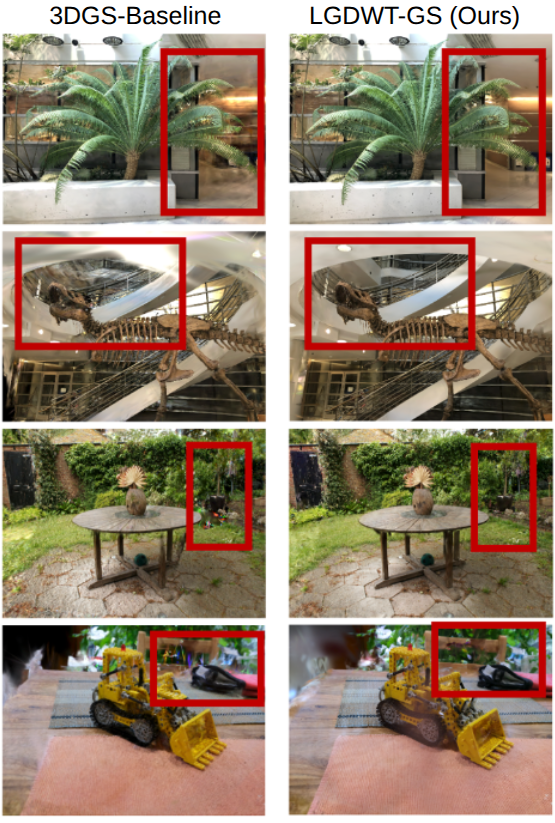
\includegraphics[width=\columnwidth]{sections/image/result.png}
  \caption{Qualitative comparison between baseline 3DGS and our LGDWT-GS on LLFF and MipNeRF360. Red boxes highlight regions with better preservation of fine details (foliage, edges, thin structures).}
  \label{fig:qualitative}
\end{figure}
\vspace{-0.6\baselineskip}

% \begin{figure}[!t]
%   \centering
%   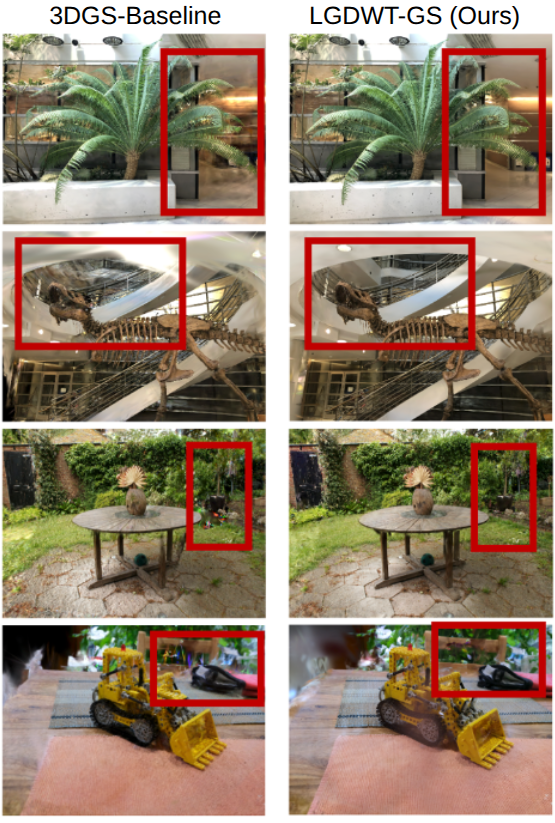
\includegraphics[width=\columnwidth,height=0.72\textheight,keepaspectratio]{sections/image/result.png}
%   \caption{Qualitative comparison between baseline 3DGS and our LGDWT-GS on LLFF and MipNeRF360. Red boxes highlight regions with better preservation of fine details (foliage, edges, thin structures).}
%   \label{fig:qualitative}
% \end{figure}

To validate LGDWT-GS in a realistic agricultural setting, we evaluated it on our custom multispectral greenhouse dataset. Each plant was captured from ten viewpoints using synchronized RGB and NIR cameras. Table~\ref{tab:multispectral_results} compares the performance against single-channel and standard multispectral baselines. Notably, unlike the LLFF and MipNeRF 360 experiments where high-frequency subbands were excluded, here we explicitly utilized high-frequency regularization. Since the background is irrelevant for this application, we tuned the parameters to focus on the HF components of the plant structure. This targeted approach allows the model to recover fine details, such as leaf veins, without being constrained by background noise. Consequently, LGDWT-GS consistently achieves the highest reconstruction quality across all scenes.

% \begin{table*}[!t]
% \caption{Quantitative Results on the Multispectral Greenhouse Dataset}
% \label{tab:multispectral_results}
% \centering
% \begin{tabular}{lcccccccccccc}
% \hline
% \multirow{2}{*}{Scene} &
% \multicolumn{3}{c}{Single-Channel} &
% \multicolumn{3}{c}{Single-Channel + DWT} &
% \multicolumn{3}{c}{Multispectral (no DWT)} &
% \multicolumn{3}{c}{Multispectral + DWT} \\
% \cline{2-4}\cline{5-7}\cline{8-10}\cline{11-13}
% & PSNR (dB)$\uparrow$ & SSIM$\uparrow$ & LPIPS$\downarrow$
% & PSNR (dB)$\uparrow$ & SSIM$\uparrow$ & LPIPS$\downarrow$
% & PSNR (dB)$\uparrow$ & SSIM$\uparrow$ & LPIPS$\downarrow$
% & PSNR (dB)$\uparrow$ & SSIM$\uparrow$ & LPIPS$\downarrow$ \\
% \hline
% Cotton      & 28.74 & 0.820 & 0.422 & 28.96 & 0.829 & 0.424 & 30.55 & 0.873 & \textbf{0.256} & \textbf{30.68} & \textbf{0.874} & 0.258 \\
% Grape       & 29.93 & 0.888 & 0.361 & 29.28 & 0.843 & 0.362 & 30.62 & \textbf{0.926} & 0.176 & \textbf{31.01} & 0.925 & \textbf{0.175} \\
% Sorghum     & 28.06 & 0.738 & 0.555 & 28.24 & 0.741 & 0.555 & 30.57 & 0.890 & 0.402 & \textbf{31.08} & \textbf{0.894} & \textbf{0.399} \\
% Tomato      & 26.65 & 0.788 & 0.357 & 27.08 & 0.802 & 0.351 & 29.33 & 0.885 & \textbf{0.212} & \textbf{29.59} & \textbf{0.892} & 0.213 \\
% Houseplant  & 29.36 & 0.831 & 0.417 & 28.43 & 0.799 & 0.421 & 29.24 & 0.875 & \textbf{0.245} & \textbf{29.43} & \textbf{0.875} & 0.247 \\
% \hline
% Average     & 28.55 & 0.813 & 0.422 & 28.39 & 0.802 & 0.422 & 30.06 & 0.890 & 0.258 & \textbf{30.51} & \textbf{0.892} & \textbf{0.258} \\
% \hline
% \end{tabular}
% \end{table*}

\begin{table*}[t]
\centering
\caption{Quantitative results on the multispectral greenhouse dataset.}
\label{tab:multispectral_results}
\resizebox{\textwidth}{!}{
\begin{tabular}{|c|ccc|ccc|ccc|ccc|}
\hline
Scene &
\multicolumn{3}{c|}{\textbf{Single}} &
\multicolumn{3}{c|}{\textbf{Single + DWT}} &
\multicolumn{3}{c|}{\textbf{Multispectral}} &
\multicolumn{3}{c|}{\textbf{Multispectral + DWT}} \\
\cline{2-13}
& PSNR↑ & SSIM↑ & LPIPS↓ 
& PSNR↑ & SSIM↑ & LPIPS↓ 
& PSNR↑ & SSIM↑ & LPIPS↓ 
& PSNR↑ & SSIM↑ & LPIPS↓ \\
\hline
Cotton     & 28.74 & 0.820 & 0.422 & 28.96 & 0.829 & 0.424 & 30.55 & 0.873 & \textbf{0.256} & \textbf{30.68} & 0.874 & 0.258 \\
Grape      & 29.93 & 0.888 & 0.361 & 29.28 & 0.843 & 0.362 & 30.62 & \textbf{0.926} & 0.176 & \textbf{31.01} & 0.925 & \textbf{0.175} \\
Sorghum    & 28.06 & 0.738 & 0.555 & 28.24 & 0.741 & 0.555 & 30.57 & 0.890 & 0.402 & \textbf{31.08} & 0.894 & \textbf{0.399} \\
Tomato     & 26.65 & 0.788 & 0.357 & 27.08 & 0.802 & 0.351 & 29.33 & 0.885 & \textbf{0.212} & \textbf{29.59} & 0.892 & 0.213 \\
Houseplant & 29.36 & 0.831 & 0.417 & 28.43 & 0.799 & 0.421 & 29.24 & 0.875 & \textbf{0.245} & \textbf{29.43} & 0.875 & 0.247 \\
\hline
\textbf{Average} & 28.55 & 0.813 & 0.422 & 28.39 & 0.802 & 0.422 & 30.06 & 0.890 & 0.258 & \textbf{30.51} & \textbf{0.892} & \textbf{0.258} \\
\hline
\end{tabular} }
\end{table*}

% \begin{table*}[t]
% \centering
% \caption{Quantitative results on the multispectral greenhouse dataset.}
% \resizebox{\textwidth}{!}{
% \begin{tabular}{lcccccccccccc}
% \toprule
% \multirow{2}{*}{Scene} &
% \multicolumn{3}{c}{Single} &
% \multicolumn{3}{c}{Single + DWT} &
% \multicolumn{3}{c}{Multi} &
% \multicolumn{3}{c}{Multi + DWT} \\
% & PSNR↑ & SSIM↑ & LPIPS↓ &
%   PSNR↑ & SSIM↑ & LPIPS↓ &
%   PSNR↑ & SSIM↑ & LPIPS↓ &
%   PSNR↑ & SSIM↑ & LPIPS↓ \\
% \midrule
% Cotton     & 28.74 & 0.820 & 0.422 & 28.96 & 0.829 & 0.424 & 30.55 & 0.873 & \textbf{0.256} & \textbf{30.68} & 0.874 & 0.258 \\
% Grape      & 29.93 & 0.888 & 0.361 & 29.28 & 0.843 & 0.362 & 30.62 & \textbf{0.926} & 0.176 & \textbf{31.01} & 0.925 & \textbf{0.175} \\
% Sorghum    & 28.06 & 0.738 & 0.555 & 28.24 & 0.741 & 0.555 & 30.57 & 0.890 & 0.402 & \textbf{31.08} & 0.894 & \textbf{0.399} \\
% Tomato     & 26.65 & 0.788 & 0.357 & 27.08 & 0.802 & 0.351 & 29.33 & 0.885 & \textbf{0.212} & \textbf{29.59} & 0.892 & 0.213 \\
% Houseplant & 29.36 & 0.831 & 0.417 & 28.43 & 0.799 & 0.421 & 29.24 & 0.875 & \textbf{0.245} & \textbf{29.43} & 0.875 & 0.247 \\
% \midrule
% Average    & 28.55 & 0.813 & 0.422 & 28.39 & 0.802 & 0.422 & 30.06 & 0.890 & 0.258 & \textbf{30.51} & \textbf{0.892} & \textbf{0.258} \\
% \bottomrule
% \end{tabular}
% }
% \end{table*}





\subsection{Qualitative Analysis}

Figure~\ref{fig:qualitative} presents qualitative comparisons between baseline 3DGS and our LGDWT-GS on standard benchmarks.  
Frequency-aware supervision improves detail preservation, notably in foliage, edges, and thin structures.  
Under sparse views, standard 3DGS often exhibits texture blurring or missing details, while LGDWT-GS retains spectral and spatial coherence.  
This qualitative trend is consistent across LLFF and MipNeRF360 datasets.


Figure~\ref{fig:multi_compare} presents a qualitative comparison on the multispectral greenhouse dataset to analyze the respective contributions of spectral diversity and frequency-domain supervision. We evaluate four reconstruction settings. The single-channel baseline exhibits over-smoothed textures and distorted edges due to limited spectral information. Incorporating DWT improves edge sharpness but does not fully resolve geometric inconsistencies. In contrast, multispectral training enhances global structural stability, though fine details remain blurred. By combining both components, LGDWT-GS achieves the best overall performance, producing sharp and coherent reconstructions with well-preserved leaf boundaries and minimal artifacts. These results demonstrate that spectral diversity promotes geometric stability, while frequency supervision effectively recovers HF details.

\begin{figure*}[!t]
    \centering
    
    \subfloat[]{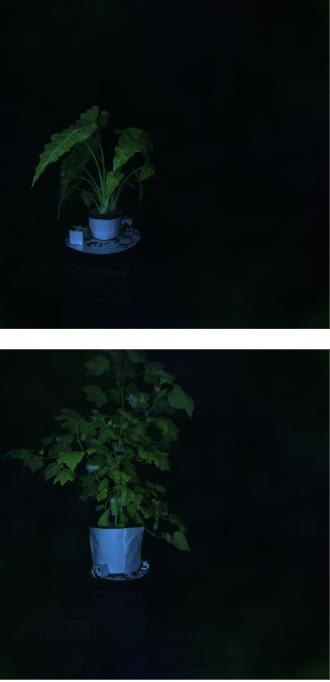
\includegraphics[width=0.18\textwidth]{sections/image/111.png}\label{fig_gt}}
    \hfill
    \subfloat[]{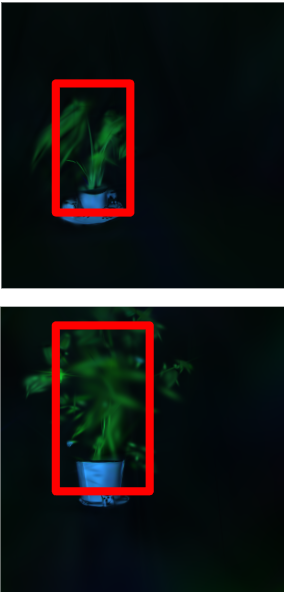
\includegraphics[width=0.18\textwidth]{sections/image/222.png}\label{fig_sc}}
    \hfill
    \subfloat[]{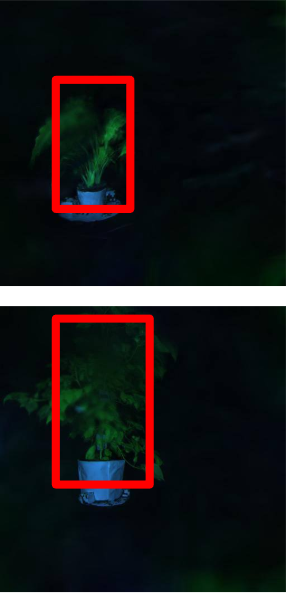
\includegraphics[width=0.18\textwidth]{sections/image/333.png}\label{fig_sc_dwt}}
    \hfill
    \subfloat[]{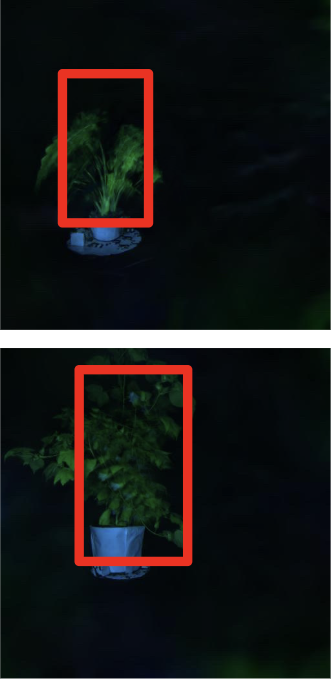
\includegraphics[width=0.18\textwidth]{sections/image/444.png}\label{fig_ms}}
    \hfill
    \subfloat[]{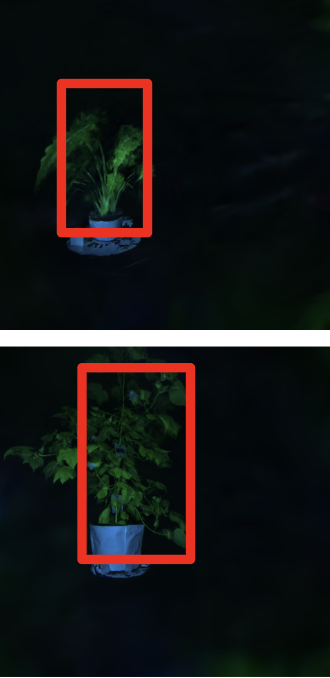
\includegraphics[width=0.18\textwidth]{sections/image/555.png}\label{fig_ms_dwt}}

    \caption{
        Comparison of reconstruction outputs across input configurations:  
        (a) Ground Truth,  
        (b) Single-channel,  
        (c) Single-channel + DWT,  
        (d) Multispectral (no DWT),  
        (e) Multispectral + DWT.  
    }
    \label{fig:multi_compare}
\end{figure*}




% \subsection{Ablation Study}
% \label{sec:ablation}

% We evaluated the contribution of each component in the proposed framework through systematic ablations under the 3-view LLFF configuration. As an edge-aware baseline, the NEHD loss combines responses from multiple edge detection operators to emphasize high-contrast structures and provide a reference point for evaluating frequency-domain supervision. The baseline DWT loss introduces frequency-domain supervision through four subbands (LL, LH, HL, HH), improving structural consistency. Adding depth regularization further refines geometric accuracy and stabilizes Gaussian placement by leveraging depth priors. Staged DWT training progressively activates subbands during optimization, stabilizing convergence and preventing early HF artifacts. The two-level DWT decomposition extends supervision to multiple scales, improving multi-frequency consistency but slightly smoothing fine textures due to the dominance of low-frequency emphasis. Finally, combining global and local DWT supervision provides the most balanced performance, reinforcing both coarse structural stability and fine texture recovery by aligning global frequency coherence with localized refinement. Overall, the results in Table~\ref{tab:ablation} confirm that frequency-aware supervision significantly enhances sparse-view reconstruction, with the global–local configuration achieving the most stable and detail-preserving results.

% \begin{table}[!t]
% \caption{Ablation Study on LLFF (3-View) Scenes}
% \label{tab:ablation}
% \centering
% \begin{tabular}{lcccc}
% \hline
% Configuration        & PSNR (dB)$\uparrow$ & SSIM$\uparrow$ & LPIPS$\downarrow$ & Time (s) \\ \hline
% NEHD Loss            & 19.99               & 0.755          & 0.268             & $\sim$360 \\
% DWT Loss             & 19.92               & 0.680          & 0.314             & $\sim$120 \\
% DWT + Depth Reg.     & 20.03               & 0.683          & 0.304             & $\sim$126 \\
% DWT Staging          & 20.08               & 0.720          & 0.298             & $\sim$120 \\
% Two-Level DWT        & 20.28               & 0.726          & 0.297             & $\sim$166 \\
% Global + Local DWT   & 20.46               & 0.726          & 0.279             & $\sim$166 \\ \hline
% \end{tabular}
% \end{table}

\subsection{Ablation Study}
\label{sec:ablation}

To isolate the contribution of frequency-domain supervision, we conducted a systematic component analysis on the 3-view LLFF configuration (Table~\ref{tab:ablation}). We compared our method against Neural Edge Histogram Descriptors (NEHD)~\cite{peeples2025histogram}. NEHD uses Sobel kernels \cite{sobel19683x3} to extract edge responses and aggregates the responses using differentiable histograms of gradient magnitudes to align the edge distributions of rendered and ground-truth images to improve texture representations. During optimization, NEHD explicitly focuses the rendering loss on HF edge regions. By heavily weighting these fine detail boundaries, NEHD forces the model to prioritize sharp discontinuities, achieving a PSNR of 19.99 dB. However, this aggressive focus on edges creates a trade-off: while it sharpens high-contrast boundaries, it often treats subtle surface textures like leaf veins as noise or fails to register them if they lack strong gradient magnitude. This results in reconstructions with sharp outlines but ``waxy", over-smoothed interiors.

In contrast to NEHD, LGDWT-GS employs a DWT loss to supervise the entire frequency spectrum. While NEHD treats non-edge pixels uniformly, the DWT decomposes the signal into distinct sub-bands, effectively decoupling global structure from fine texture. This allows the model to enforce structural consistency through LF bands while simultaneously recovering detailed textures via HF bands even in regions with weak spatial gradients. Furthermore, in sparse-view settings, the DWT acts as a soft regularizer, suppressing HF artifacts in empty space while preserving valid signals in textured areas.

The component analysis highlights the specific contributions of our architectural choices. Depth regularization improves PSNR by 0.11 dB by stabilizing geometry and preventing Gaussians from drifting near the camera, a common failure in sparse SfM initialization. Additionally, employing a two-level decomposition with progressive frequency staging enables the model to establish coarse geometry before refining fine details, thereby preventing early convergence to local minima. Finally, combining global structural constraints with patch-based local refinement yields the most balanced performance, achieving the highest SSIM of 0.726 and an LPIPS of 0.279.


\begin{table}[!t]
\caption{Ablation Study on LLFF (3-View) Scenes}
\label{tab:ablation}
\centering
\begin{tabular}{lcccc}
\hline
Configuration        & PSNR (dB)$\uparrow$ & SSIM$\uparrow$ & LPIPS$\downarrow$ & Time (s) \\ \hline
NEHD Loss            & 19.99               & 0.755          & 0.268             & $\sim$360 \\
DWT Loss             & 19.92               & 0.680          & 0.314             & $\sim$120 \\
DWT + Depth Reg.     & 20.03               & 0.683          & 0.304             & $\sim$126 \\
DWT Staging          & 20.08               & 0.720          & 0.298             & $\sim$120 \\
Two-Level DWT        & 20.28               & 0.726          & 0.297             & $\sim$166 \\
Global + Local DWT   & 20.46               & 0.726          & 0.279             & $\sim$166 \\ \hline
\end{tabular}
\end{table}
% \subsection{Discussion}

% In general, our experiments demonstrate that LGDWT-GS effectively bridges the gap between geometric and frequency-domain supervision.  
% In few-view and multispectral setups, it delivers sharper, more coherent reconstructions while maintaining stability across spectral bands.  
% Performance gains are most significant in sparse regimes, confirming that frequency domain priors act as strong regularizers when spatial information is limited.  
% As the number of input views increases, the marginal benefit of DWT regularization diminishes, suggesting its greatest utility in data-constrained reconstruction scenarios.
